One of the key challenges in protein design is modeling and searching the many continuous conformational degrees of freedom inherent in proteins and other molecules. The sidechain conformations of each amino-acid type are generally found in clusters, known as rotamers~\cite{rotamers}, so it is common practice to approximate protein conformational space as discrete by forcing each residue to be in the modal conformation of one of these clusters~\cite{DEE,DEE/A*}.  However, design accuracy is increased significantly when continuous flexibility is taken into account, by allowing the continuous degrees of freedom to move within finite bounds around these modal values~\cite{iMinDEE,DEEPer,OSPREY_MIE,BBK*}.  Moreover, this increase in accuracy depends on considering continuous flexibility~\textit{during} the conformational search process, rather than simply performing minimization~\textit{post hoc} on the top-scoring sequences and conformations output by a discrete search algorithm.  Although such a~\textit{post hoc} minimization approach would obtain more energetically favorable models of the top sequences, it would still produce the same top sequences as a purely discrete design would, which may not be truly the top sequences.  For example, clashing discrete rotamers can often be converted to favorable conformations by relatively small adjustments in the sidechain conformations~\cite{minDEE,iMinDEE,DEEPer,CATS}.  As a result, designs performed with continuous flexibility taken into account~\textit{throughout the search} yield significantly different, and more biologically accurate, sequences than the same designs performed using discrete search~\cite{iMinDEE,DEEPer,OSPREY_MIE}.  

To address this problem, \osprey includes several algorithms to design proteins while taking continuous flexibility into account throughout the process of sequence and conformational search~\cite{minDEE,iMinDEE,DEEPer,EPIC,LUTE_RECOMB,CATS}.   These algorithms predict optimal protein sequences with provable guarantees of accuracy given a biophysical model that includes continuous flexibility.  

This~\textit{minimization-aware} design approach requires energy minimization to be performed for a large number of conformations (within the bounds on the continuous degree of freedom that define each conformation).  This minimization is a relatively expensive operation, so the bulk of a design's runtime can be spent on energy minimization of conformations. Therefore, improvements to the speed of energy minimization can have a dramatic impact on \osprey runtimes.  

Much work has been done to optimize \osprey for execution on CPUs, particularly highly multi-core CPUs and even networked clusters of CPU-powered servers~\cite{minBounds_DACS,cloud_OSPREY}. However, modern GPU hardware enables high-performance computation for some specific tasks at a fraction of the cost of large CPU clusters, mainly due to the huge video game industry that propels innovation in hardware design and drives down costs. The widespread adoption of fast and highly programmable GPUs in the past decade has transformed many areas of computational science, including quantum chemistry~\cite{GPU_QM}, computer vision~\cite{ResNet}, and cryptography~\cite{GPU_crypto}.  In particular, GPUs have been found to produce speedups of approximately an order of magnitude in molecular dynamics simulations~\cite{HOOMD_GPU,AMBER_GPU_microseconds,GROMACS_GPU}, which, like \osprey, must sum huge numbers of forcefield energy terms and can use the GPU to parallelize this computation.  

Thus, in order to bring the benefit of GPUs to protein design calculations, \osprey 3.0 includes GPU programs (called {\it kernels}) built using the CUDA framework~\cite{nvidia2010programming} that implement the forcefield calculations and local minimization algorithms used in protein redesign.

We present performance results of these GPU kernels on various hardware platforms in Figure~\ref{fig:gpu}. A GPU server housing 4 Nvidia Tesla P100 cards can finish minimizations with about 300,000 atom pairs roughly 110-fold faster than a single thread running on an Intel Xeon E5-2640 v4 CPU. With two Intel Xeon E5-2640 v4 CPUs running at full capacity with multiple threads, the four Nvidia Tesla P100 GPUs finish the same minimizations roughly 8-fold faster. The speedups of GPUs over CPUs scale with the number of atom pairs in the minimization. For minimizations with fewer (about 30,000) atom pairs, even four Nvidia Tesla P100 GPUs cannot outperform two Intel Xeon E5-2640 v4 CPUs. There is significant overhead to transfer each minimization problem from the CPU to the GPU during designs. Even though GPUs can evaluate the minimizations much faster than CPUs, when there are few atom pairs, this transfer overhead dominates the computation time and causes GPUs to perform merely similarly to CPUs, rather than significantly faster.  Nevertheless, the bottleneck in protein design is minimizations with many atom pairs, and for these minimizations \osprey's speedups on GPUs are on par with the state of the art for GPU speedups of molecular dynamics simulations.  

The performance of desktop hardware appears similar to server hardware, except on a smaller scale. A single Nvidia GTX 1070 GPU performs minimizations at roughly half the speed of an Nvidia Tesla P100 GPU. Two Nvidia GTX 1080 GPUs perform similarly to the Nvidia Tesla P100 GPU on the large conformation benchmark (Fig.~\ref{fig:gpu}, bottom), but actually perform worse than a single Nvidia GTX 1070 for the small conformation benchmark (Fig.~\ref{fig:gpu}, middle) -- despite having well over twice the hardware of the single Nvidia GTX 1070 GPU. This anomalous performance suggests the kernel \osprey 3.0 uses for minimizations is not yet well-optimized for the Nvidia GTX 1080 GPU, and that future engineering efforts could offer significant performance increases for Nvidia GTX 1080 GPUs. The Nvidia GTX 1050, a laptop GPU, does not appear to be powerful enough to offer any advantages over traditional CPU computing in \osprey 3.0 (Fig.~\ref{fig:gpu}, light blue columns).

Modern GPU architectures offer thousands of parallel hardware units for calculations, compared to the tens of parallel hardware units in modern CPU architectures. The performance results of the current generation of \osprey's GPU kernels indicate that minimization speeds on GPUs have only begun to scratch the surface of what is possible, particularly for minimizations with few atom pairs. Future versions of these GPU kernels will likely offer significantly higher performance on the same hardware -- perhaps allowing minimization speeds many times faster than today's GPU kernels.  This in turn will make it even more efficient to perform minimization-aware protein design, and allow minimization-aware designs with even more mutable and flexible residues and with more mutation options per residue.  

\begin{figure}
\center
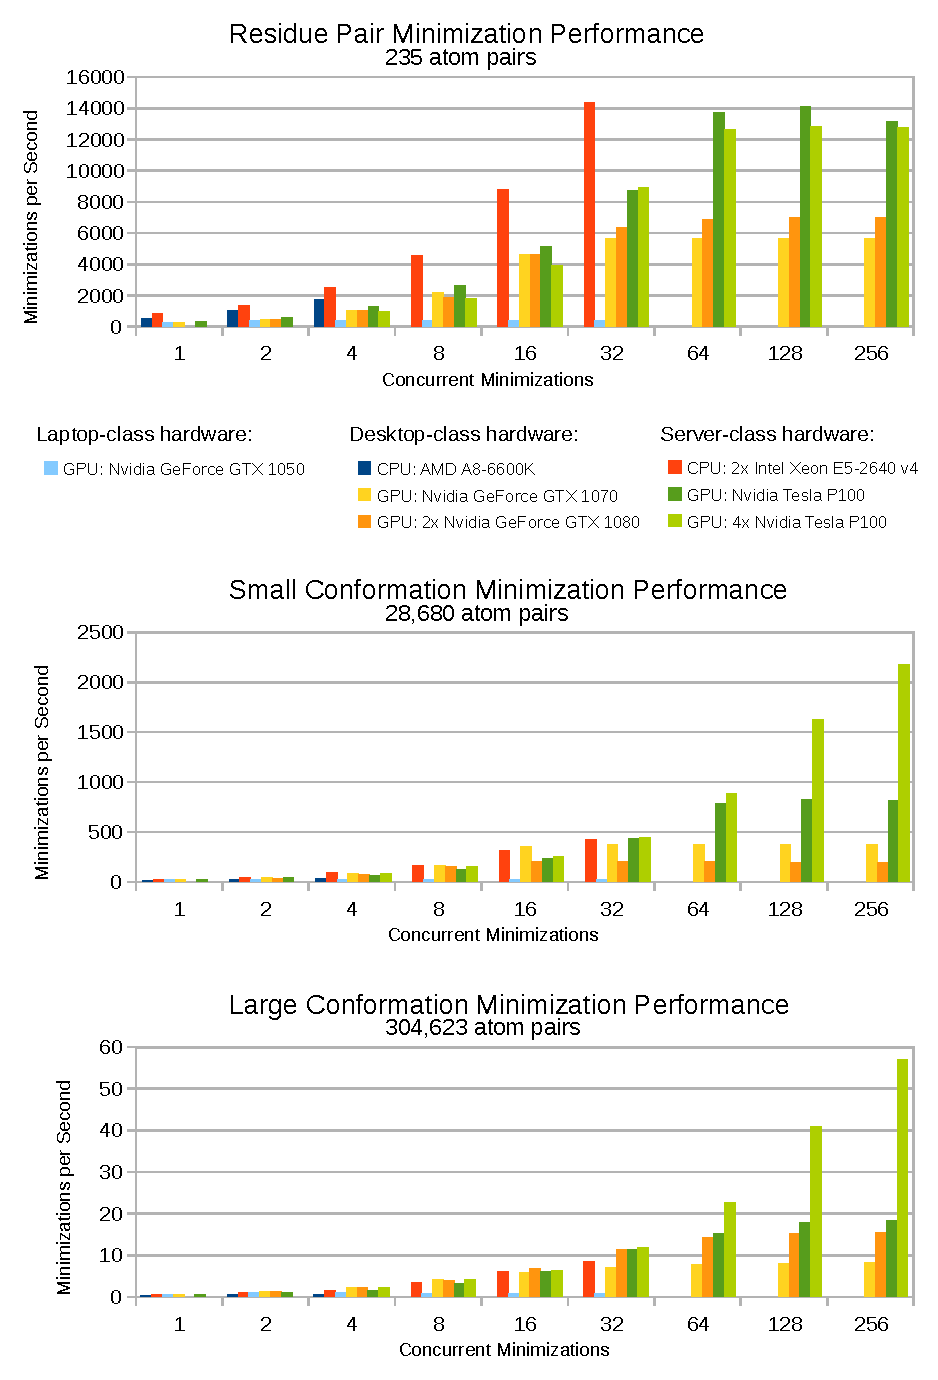
\includegraphics[width=4in]{figures/gpu.pdf}
\caption{Benchmarks for protein conformation minimization in \osprey 3.0 for various hardware platforms and for conformations of varying size. From smallest to largest: {\bf (top)} a single residue pair is the smallest multi-body minimization possible, {\bf (middle)} a full protein conformation with a single flexible residue represents a small design, {\bf (bottom)} a full protein conformation with 20 flexible residues represents a large design. For CPU hardware, concurrent minimizations correspond to CPU threads. For GPU hardware, concurrent minimizations correspond to {\it streams} defined by the CUDA framework. Faster minimization speeds correspond with faster \osprey runtimes. All minimizations were performed on the Atx1 metallochaperone protein (PDB ID: 1CC8)~\cite{1CC8}. Flexible residues were modeled with continuous sidechain flexibility, and all other residues remained completely fixed.}
\label{fig:gpu}
\end{figure}
